\section{Appendix}
our sensor is at a fixed distance from the slits with $z=0.855 [m]$.
The angle $\theta$ and the Intensity $I$ were measured using a resistor and a photodiod, the voltage on these resistors ($V\propto\theta,I$) was
measured at a rate of $40[Hz]$ and a resolution of $\Delta V\approx10^{-3}[V]$.
Prior to every measurement we align the laser beam with the sensor by detecting the point of maximum intensity, then place the slits perpendicular to
the beam.
The slits are then moved along the x axis until we measure maximum amplitude for a single slits and n slits, or between the two maxima for double slit patterns.
These procedures are key to make sure our wave is a good approximation for a plain wave and it is reaching the slits with uniform phase thus avoiding major differences from our models' assumptions.
The sensor was then moved to scan the intensities at some range of angles which were then converted to distances on our theoretical screen.
As can be seen in figure \ref{fig:single slit interference with 0.04mm width} the theory for a single slit fits the data well however there are
secondary effects easily observable in the tails of the data that per our understanding are partially caused by the non-linearity of the
photomultiplier and photoelectric sensor, such effects were not taken into account when formulating our theory
However the adjustment can be easily accomplished.
\begin{figure}[H]
    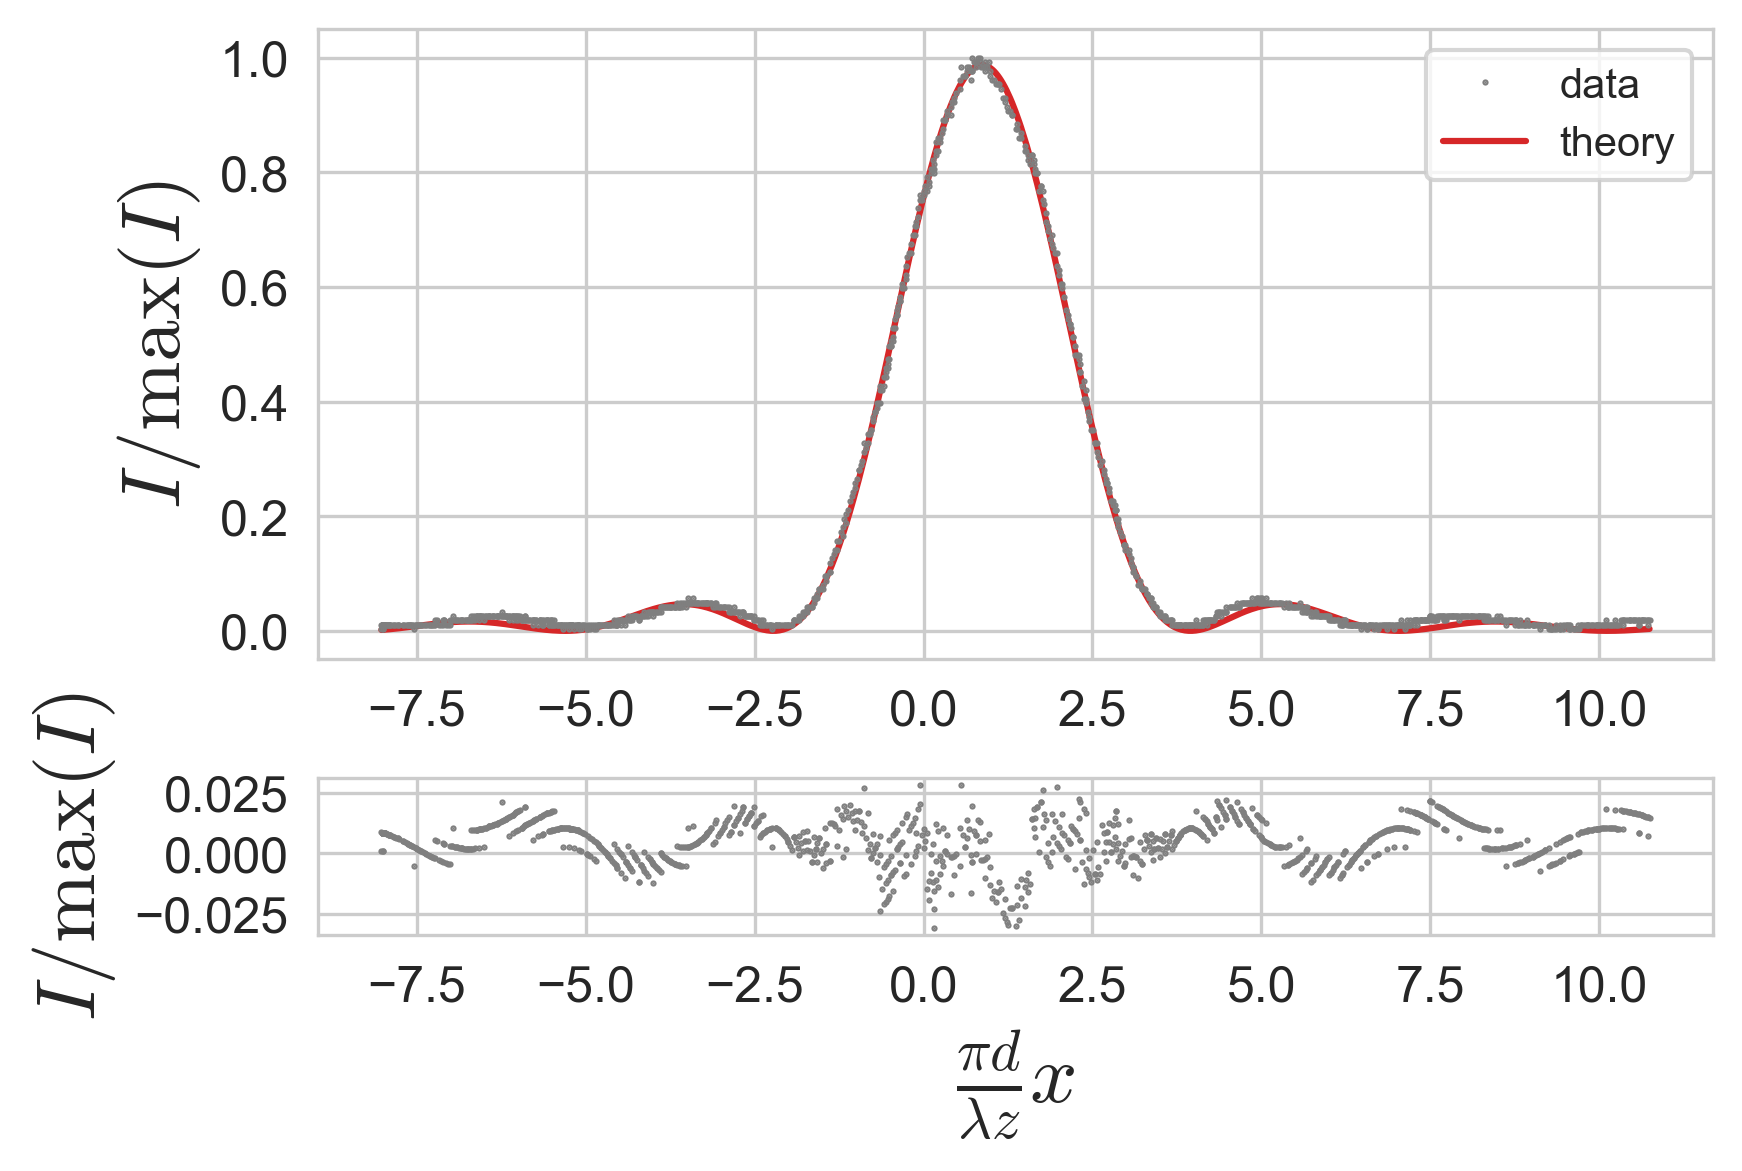
\includegraphics[width=0.9\columnwidth]{figures/single slit interference with 0.04mm width.png}
    \caption{$\lambda$ is the laser wave length $d$ is the width of the slit and $z$ is the distance from the screen}
    \label{fig:single slit interference with 0.04mm width}
\end{figure}
\begin{figure}[H]
	\centering
	\begin{subfigure}{0.5\columnwidth}
		\centering
		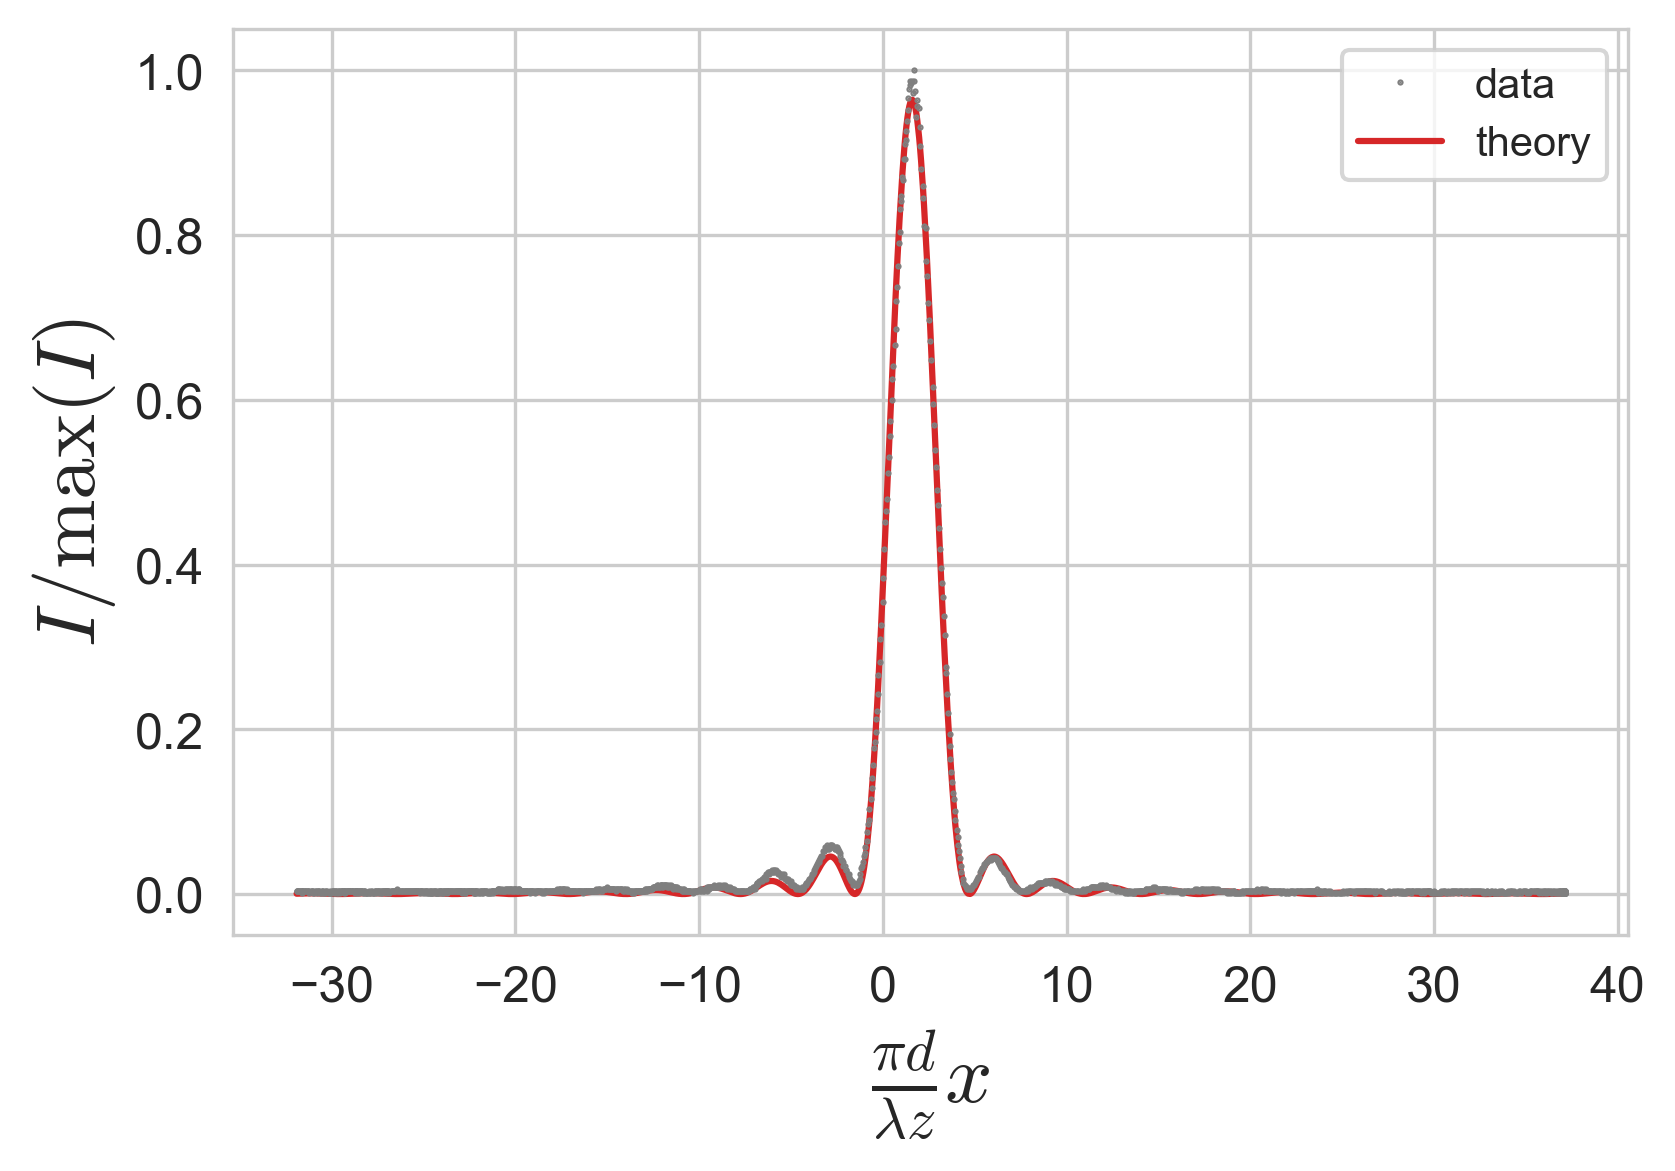
\includegraphics[width=\columnwidth]{figures/single slit interference 0.08mm.png} % first figure itself
		\caption{first figure}
        \label{fig:single slit interference 0.08mm}
	\end{subfigure}\hfill
    \begin{subfigure}{0.5\columnwidth}
        \centering
        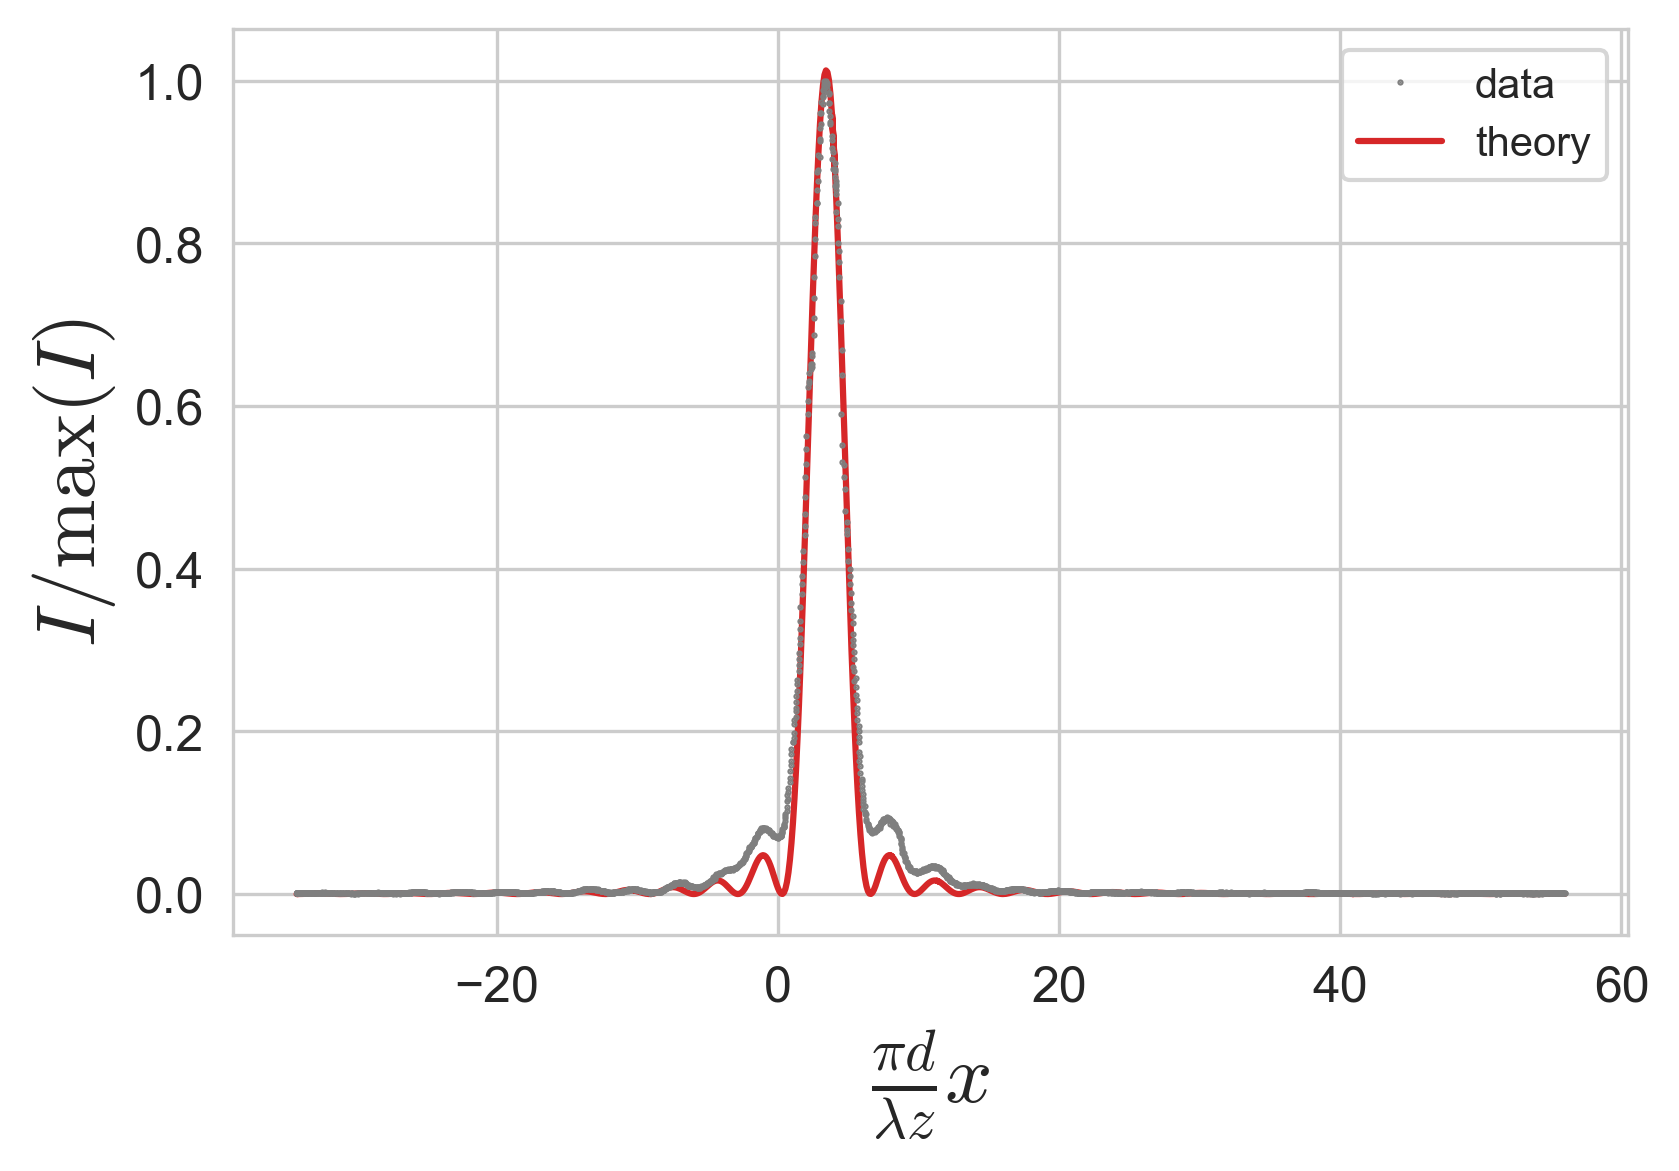
\includegraphics[width=\columnwidth]{figures/single slit interference 0.16mm.png} % second figure itself
        \caption{second figure}
        \label{fig:single slit interference 0.16mm}
    \end{subfigure}
    \label{fig:single slit examples}
\end{figure}

\begin{figure}[H]
    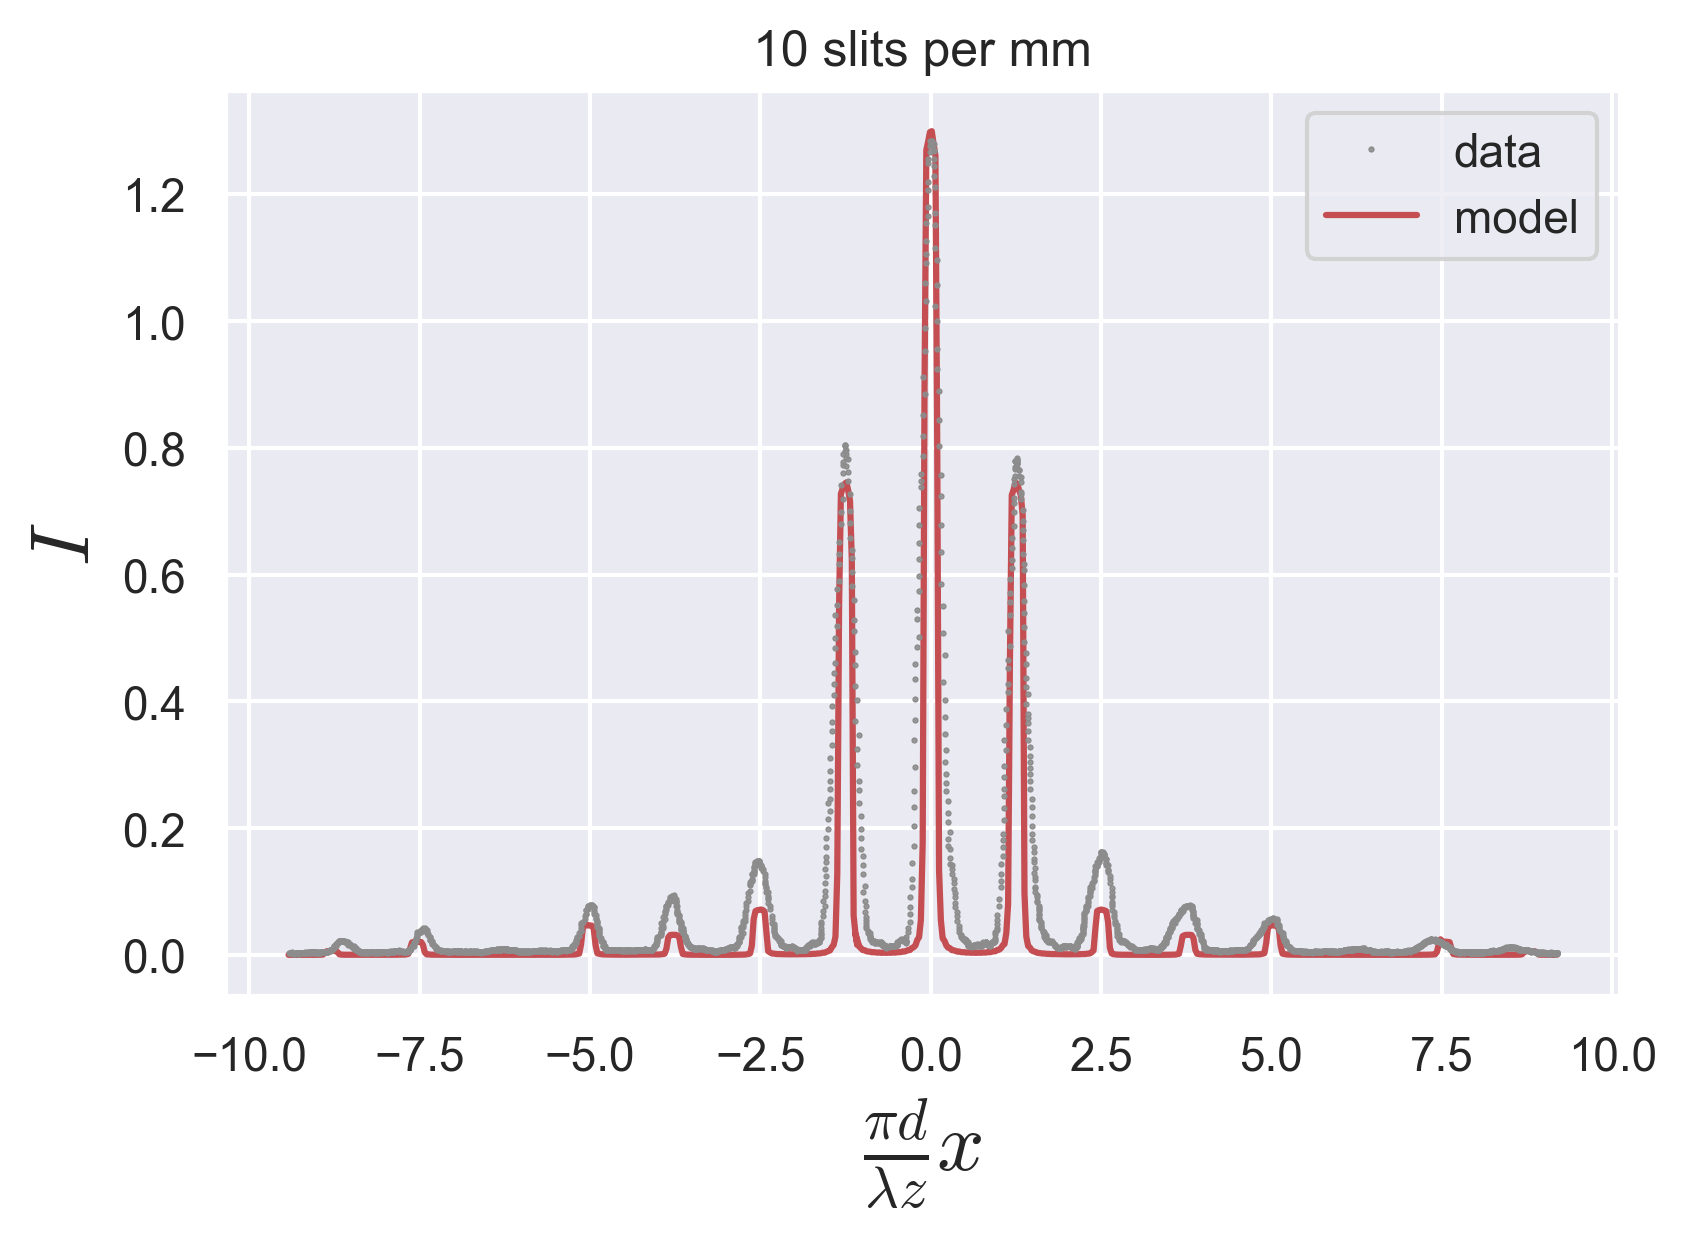
\includegraphics[width=0.9\columnwidth]{figures/10 slits per mm.png}
    \caption{}
    \label{fig:10 slits per mm}
\end{figure}
In the case of the periodic diffraction grating "10 lines per mm" the secondary effects are more pronounced especially
the photoelectric sensor's "memory" (The photoelectric sensor has a relaxation period in which to voltage diminishes
therefore after exposure instead of an immediate cut off a slope can be seen as the voltage is recorded with the relation
to the angle which continues to change during said period giving us higher peaks and wider slopes near those peaks)
\begin{figure}[H]
    \centering
    \begin{subfigure}{0.9\columnwidth}
        \centering
        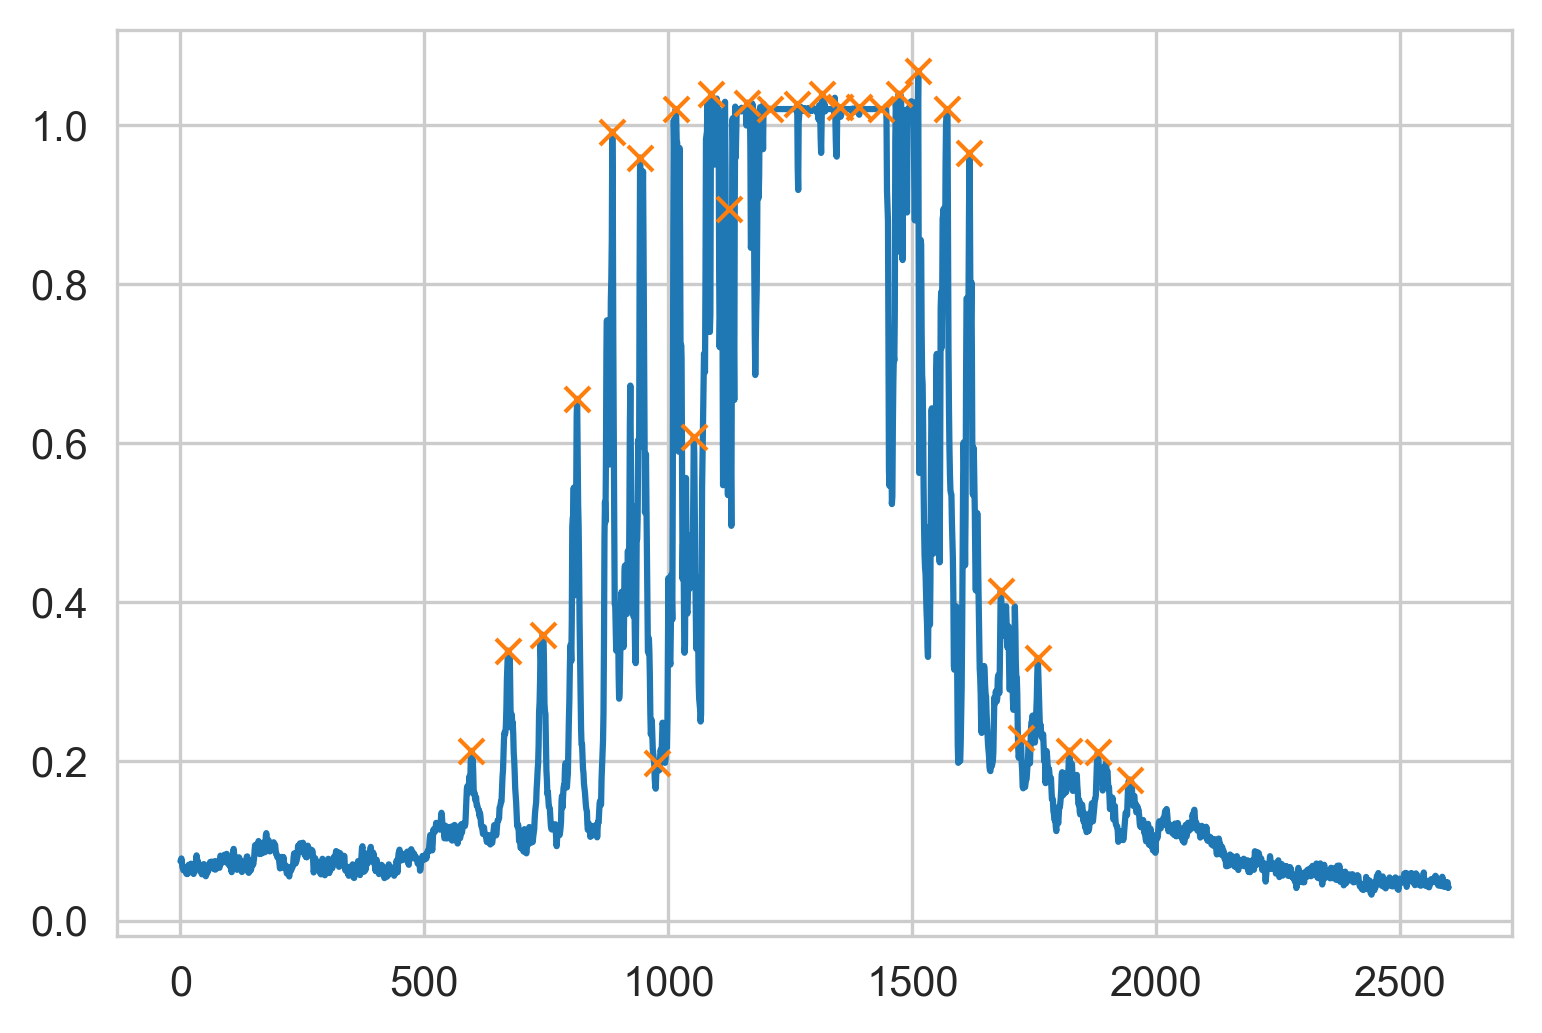
\includegraphics[width=\columnwidth]{figures/X section 1.png} % second figure itself
        \caption{"X" section 1}
        \label{fig:XSection1}
    \end{subfigure}
    \begin{subfigure}{0.9\columnwidth}
        \centering
        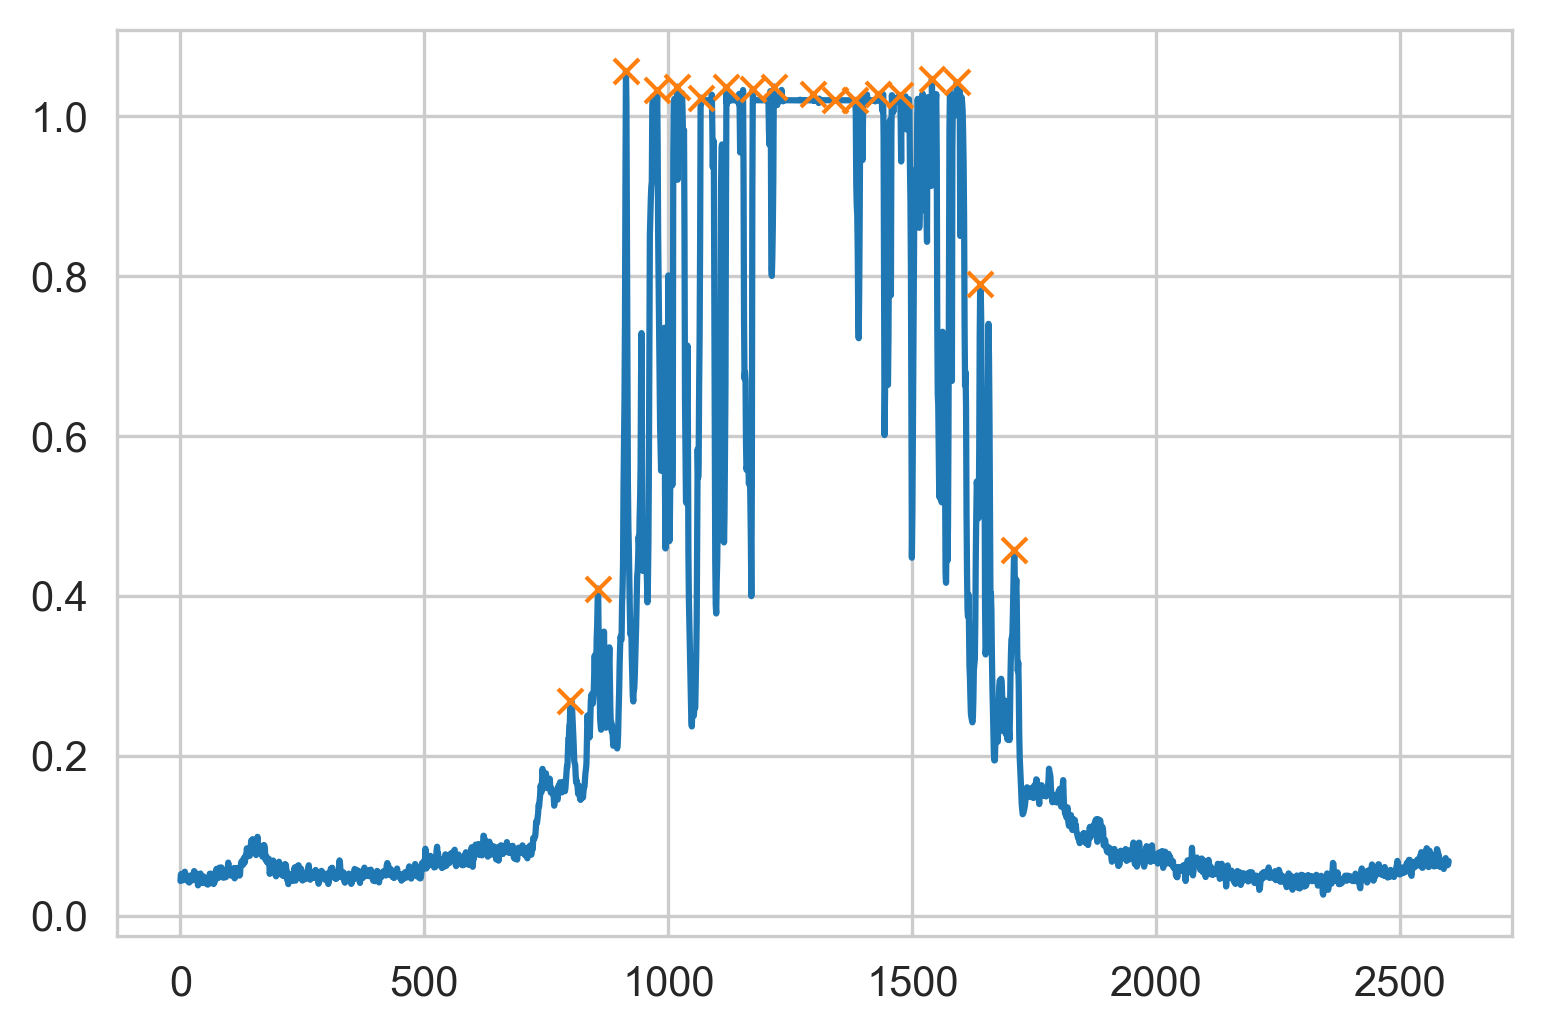
\includegraphics[width=\columnwidth]{figures/X section 2.png}
        \caption{"X" section 2}
        \label{fig:XSection2}
    \end{subfigure}
    \caption{Distances between local maxima along the "X" sections}
    \label{fig:X Sections}
\end{figure}